\documentclass{beamer}

% Beamer style
%\usetheme[secheader]{Madrid}
\usetheme{CambridgeUS}
\usecolortheme[rgb={0.65,0.15,0.25}]{structure}
%\usefonttheme[onlymath]{serif}
\beamertemplatenavigationsymbolsempty
%\AtBeginSubsection

% Packages
%\usepackage[french]{babel}
\usepackage[latin1]{inputenc}
\usepackage{color}
\usepackage{dsfont, stmaryrd}
\usepackage{amsmath, amsfonts, amssymb}
\usepackage{stmaryrd}
\usepackage{epsfig}
\usepackage{/Latex/astats}
%\usepackage[all]{xy}
\usepackage{graphicx}

% Commands
\definecolor{darkred}{rgb}{0.65,0.15,0.25}
\newcommand{\emphase}[1]{\textcolor{darkred}{#1}}
\newcommand{\paragraph}[1]{\emphase{#1}}
\newcommand{\refer}[1]{\textcolor{blue}{\sl \cite{#1}}}
\newcommand{\Refer}[1]{\textcolor{blue}{\sl #1}}
\newcommand{\newblock}{}

% Symbols
\newcommand{\Abf}{{\bf A}}
\newcommand{\Beta}{\text{B}}
\newcommand{\Bcal}{\mathcal{B}}
\newcommand{\BIC}{\text{BIC}}
\newcommand{\dd}{\text{d}}
\newcommand{\dbf}{{\bf d}}
\newcommand{\Dcal}{\mathcal{D}}
\newcommand{\Esp}{\mathbb{E}}
\newcommand{\Ebf}{{\bf E}}
\newcommand{\Ecal}{\mathcal{E}}
\newcommand{\Gcal}{\mathcal{G}}
\newcommand{\Gam}{\mathcal{G}\mbox{am}}
\newcommand{\Ibb}{\mathbb{I}}
\newcommand{\Ibf}{{\bf I}}
\newcommand{\ICL}{\text{ICL}}
\newcommand{\Cov}{\mathbb{C}\text{ov}}
\newcommand{\Corr}{\mathbb{C}\text{orr}}
\newcommand{\Var}{\mathbb{V}}
\newcommand{\Vsf}{\mathsf{V}}
\newcommand{\pen}{\text{pen}}
\newcommand{\Fcal}{\mathcal{F}}
\newcommand{\Hbf}{{\bf H}}
\newcommand{\Hcal}{\mathcal{H}}
\newcommand{\Jcal}{\mathcal{J}}
\newcommand{\Kbf}{{\bf K}}
\newcommand{\Lcal}{\mathcal{L}}
\newcommand{\Mcal}{\mathcal{M}}
\newcommand{\mbf}{{\bf m}}
\newcommand{\mum}{\mu(\mbf)}
\newcommand{\Ncal}{\mathcal{N}}
\newcommand{\Nbf}{{\bf N}}
\newcommand{\Nm}{N(\mbf)}
\newcommand{\Ocal}{\mathcal{O}}
\newcommand{\Obf}{{\bf 0}}
\newcommand{\Omegas}{\underset{s}{\Omega}}
\newcommand{\Pbf}{{\bf P}}
\newcommand{\Pcal}{\mathcal{P}}
\newcommand{\Qcal}{\mathcal{Q}}
\newcommand{\Rbb}{\mathbb{R}}
\newcommand{\Rcal}{\mathcal{R}}
\newcommand{\sbf}{{\bf s}}
\newcommand{\Sbf}{{\bf S}}
\newcommand{\Scal}{\mathcal{S}}
\newcommand{\Ucal}{\mathcal{U}}
\newcommand{\Vcal}{\mathcal{V}}
\newcommand{\Tbf}{{\bf T}}
\newcommand{\ubf}{{\bf u}}
\newcommand{\Ubf}{{\bf U}}
\newcommand{\Wbf}{{\bf W}}
\newcommand{\xbf}{{\bf x}}
\newcommand{\Xbf}{{\bf X}}
\newcommand{\Ybf}{{\bf Y}}
\newcommand{\Zbf}{{\bf Z}}
\newcommand{\pibf}{\mbox{\mathversion{bold}{$\pi$}}}
\newcommand{\Sigmabf}{\mbox{\mathversion{bold}{$\Sigma$}}}
\newcommand{\gammabf}{\mbox{\mathversion{bold}{$\gamma$}}}
\newcommand{\mubf}{\mbox{\mathversion{bold}{$\mu$}}}
\newcommand{\nubf}{\mbox{\mathversion{bold}{$\nu$}}}
\newcommand{\Thetabf}{\mbox{\mathversion{bold}{$\Theta$}}}
\newcommand{\thetabf}{\mbox{\mathversion{bold}{$\theta$}}}
\newcommand{\BP}{\text{BP}}
\newcommand{\EM}{\text{EM}}
\newcommand{\VEM}{\text{VEM}}
\newcommand{\VBEM}{\text{VB}}
\newcommand{\cst}{\text{cst}}
\newcommand{\obs}{\text{obs}}
\newcommand{\ra}{\emphase{$\rightarrow$~}}
\newcommand{\QZ}{Q_{\Zbf}}
\newcommand{\Qt}{Q_{\thetabf}}

% Directory
\newcommand{\fighd}{/RECHERCHE/RUPTURES/Exposes/Figures}

%====================================================================
\title[Exploring the segmentation space]{Exact posterior
  distribution over the segmentation space for multiple change-point
  detection problems }

\author{G. Rigaill, E. Lebarbier, \emphase{S. Robin}}

\institute[AgroParisTech / INRA]{AgroParisTech / INRA \\
  \bigskip
  \begin{tabular}{ccccc}
    
\epsfig{file=/RECHERCHE/RESEAUX/Exposes/Figures/LogoINRA-Couleur.ps,
    width=2.5cm} & 
    \hspace{.5cm} &
    
\epsfig{file=/RECHERCHE/RESEAUX/Exposes/Figures/logagroptechsolo.eps,
    width=3.75cm} & 
    \hspace{.5cm} &
    \epsfig{file=/RECHERCHE/RESEAUX/Exposes/Figures/Logo-SSB.eps,
    width=2.5cm} \\ 
  \end{tabular} \\
  \bigskip
  }

\date[IWAP, July 2010, Madrid]{Internation Workshop on Applied
  Probability, July 2010, Madrid} 

%====================================================================

%====================================================================
%====================================================================
\begin{document}
%====================================================================
%====================================================================

%====================================================================
\frame{\titlepage}
%====================================================================

%====================================================================
\section{Copy number variation (CNV)}
\frame{ \frametitle{Copy number variations (CNV)} 
  }
%==================================================================== 
\subsection{Genomic alterations}
%==================================================================== 
\frame{ \frametitle{Copy number variations in cancer cells} 
  Genomic alterations are associated with (responsible for?) various
  types of cancers.
  $$
  \begin{tabular}{cc}
    Normal cell & Tumour cell \\
    \epsfig{file =
    \fighd/KaryotypeCancer-PH.ps, clip=,
    bbllx=325, bblly=676, bburx=468, bbury=780, scale=.9} \pause  
    &
      \epsfig{file =
    \fighd/KaryotypeCancer-PH.ps, clip=,
    bbllx=127, bblly=676, bburx=319, bbury=780, scale=.9} 
    \end{tabular}
  $$
  \refer{Hup08} %\refer{Hup�}{08}
  }

%==================================================================== 
\frame{\frametitle{Technology}
  \hspace{.6cm}
  \epsfig{file=\fighd/MicroarrayTech.ps, scale=.55,
    clip=, bbllx=21, bblly=49, bburx=574, bbury=416}
  }

%====================================================================
\frame{ \frametitle{Comparative genomic hybridization (CGH)}
  \begin{tabular}{ccccc}
    \multicolumn{3}{c}{Zoom on CGH profile} & \quad & Karyotype \\
    chrom. 1 & \quad & chrom. 17 \\
    \epsfig{file = \fighd/Karyotype-CGH-PH.ps, clip=,
      bbllx=80, bblly=617, bburx=150, bbury=700, scale=1.5}
    & &
    \epsfig{file = \fighd/Karyotype-CGH-PH.ps, clip=,
      bbllx=270, bblly=617, bburx=300, bbury=700, scale=1.5} \pause
    & &
    \epsfig{file = \fighd/Karyotype-CGH-PH.ps, clip=,
      bbllx=364, bblly=617, bburx=485, bbury=763, scale=1}
  \end{tabular}

  \refer{Hup08}
  }


%==================================================================== 
\subsection{Breakpoint detection}
%==================================================================== 
\frame{ \frametitle{A segmentation problem}
  \begin{tabular}{cc}
    Raw profile & Interpretation \\
    \\
    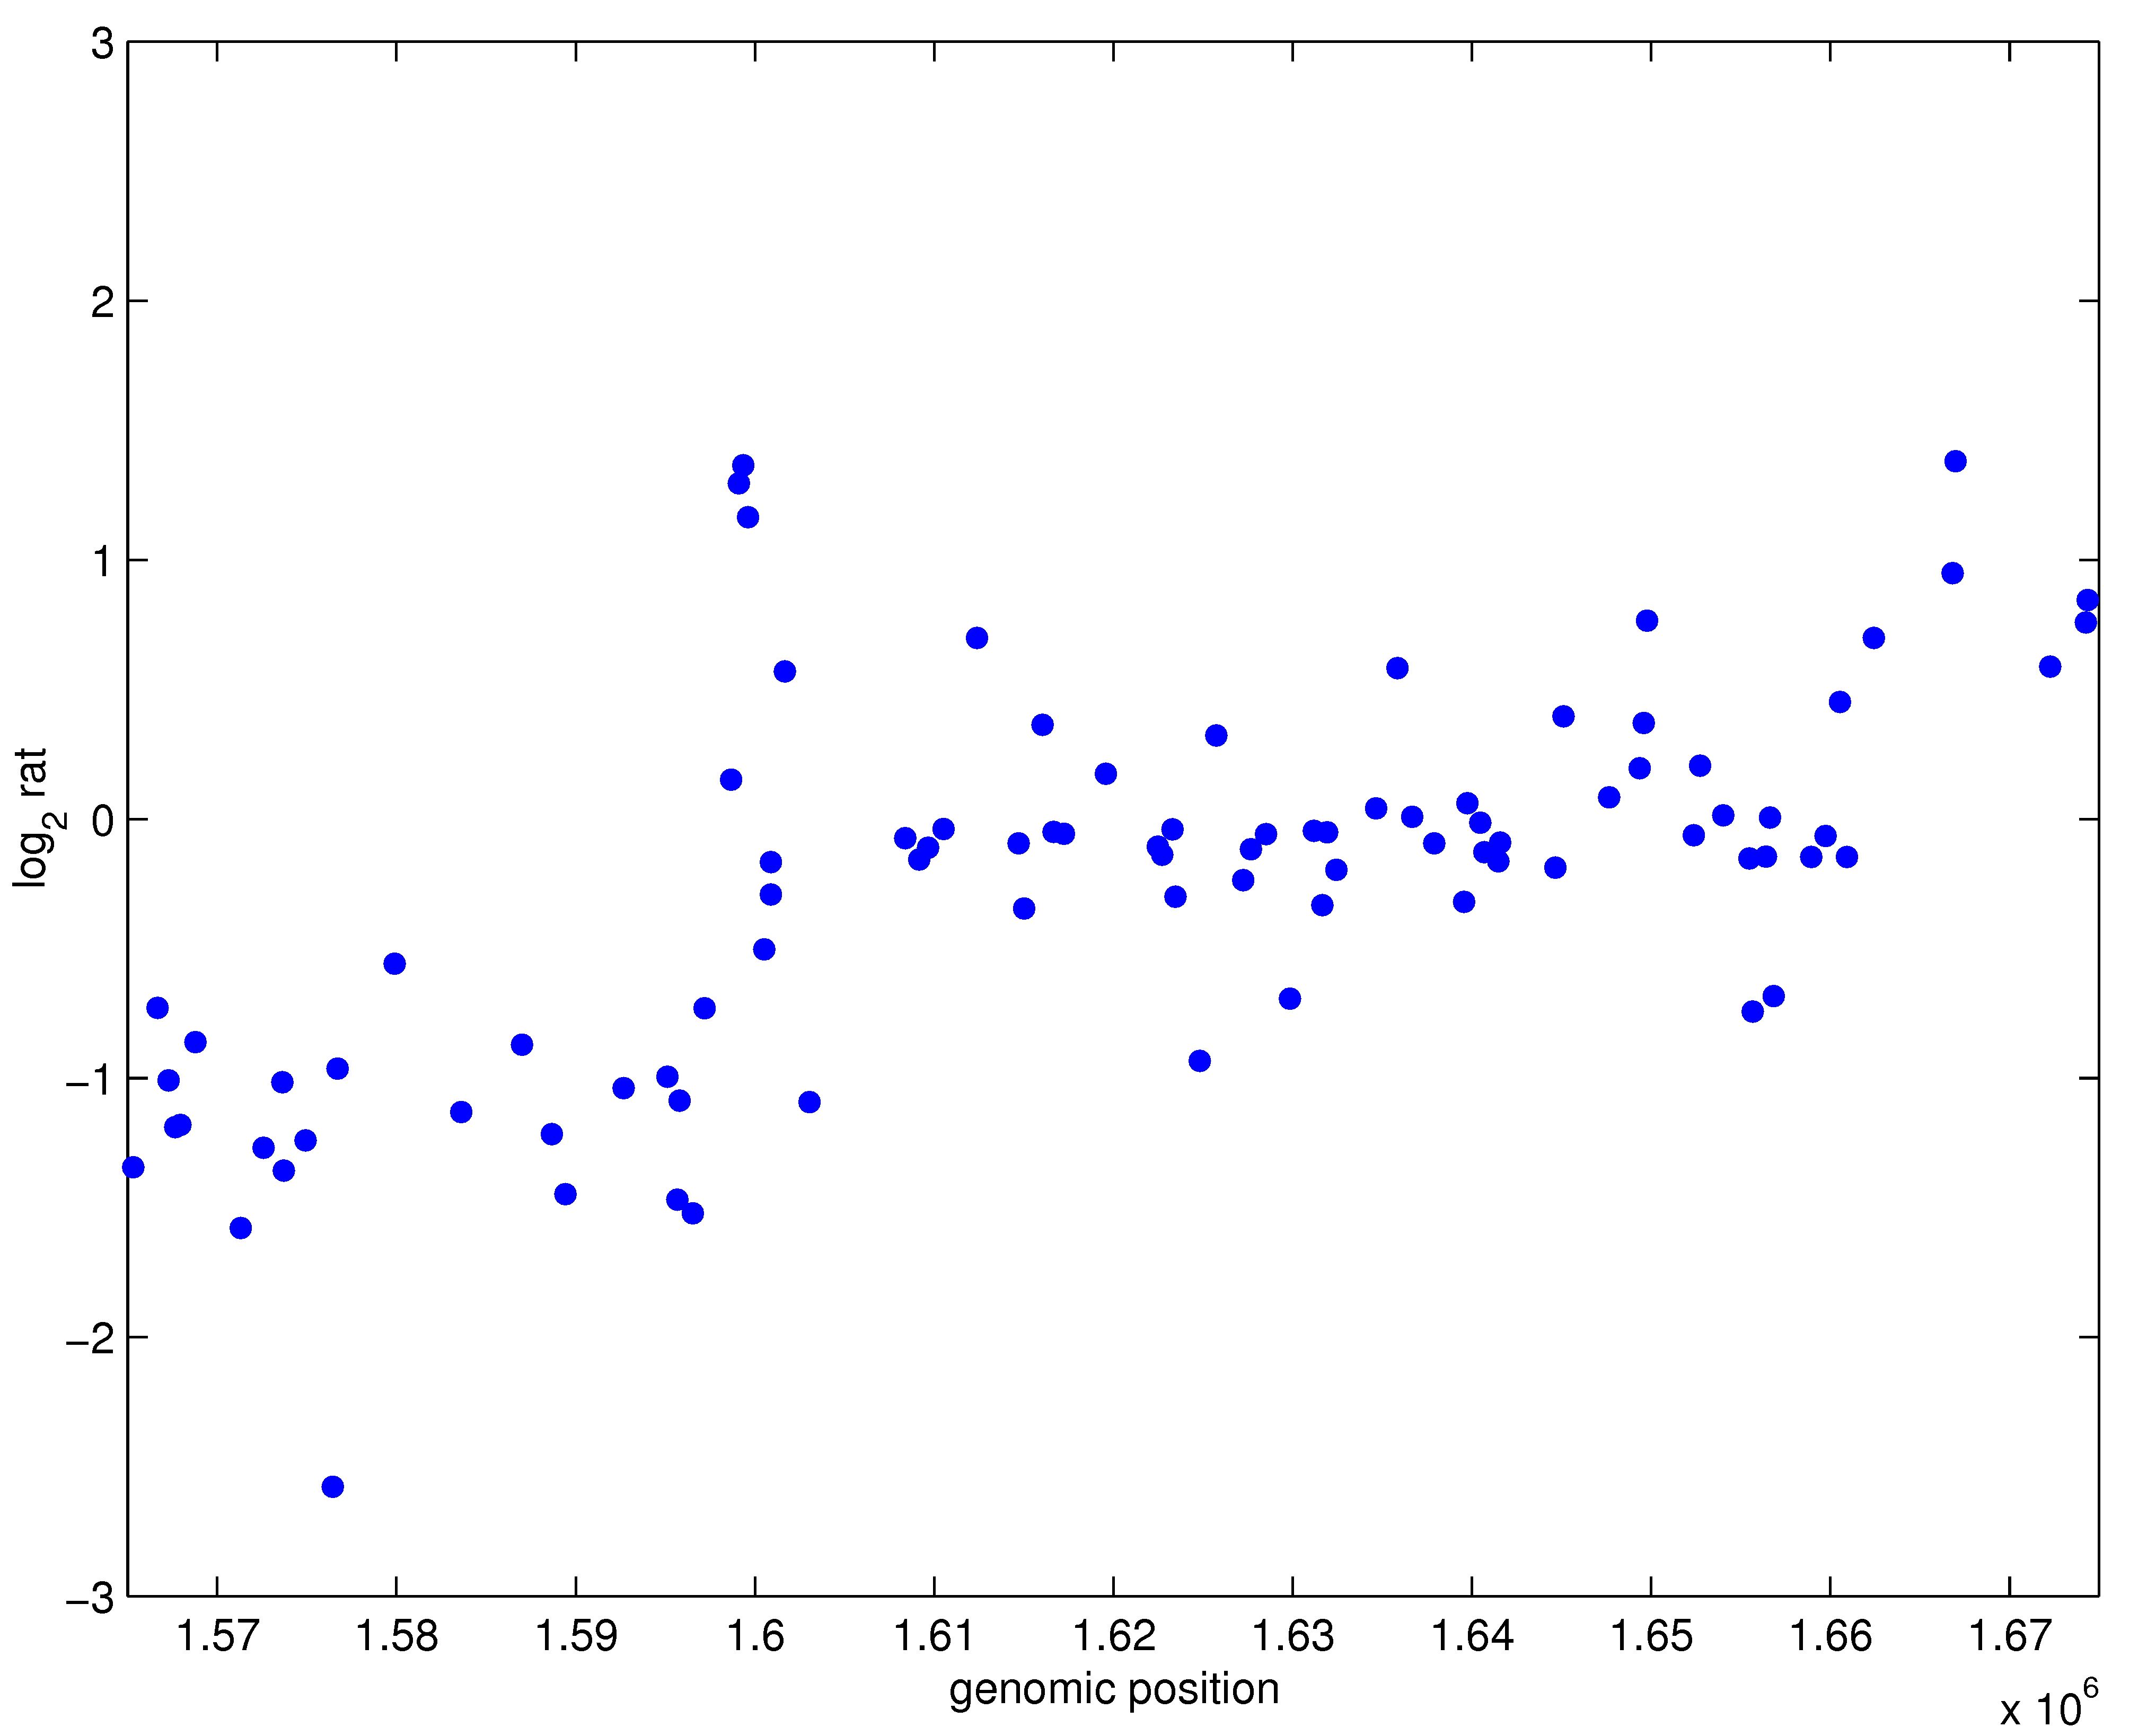
\epsfig{file = \fighd/raw_profile_example.eps, clip=, scale=.325} \pause
    &
    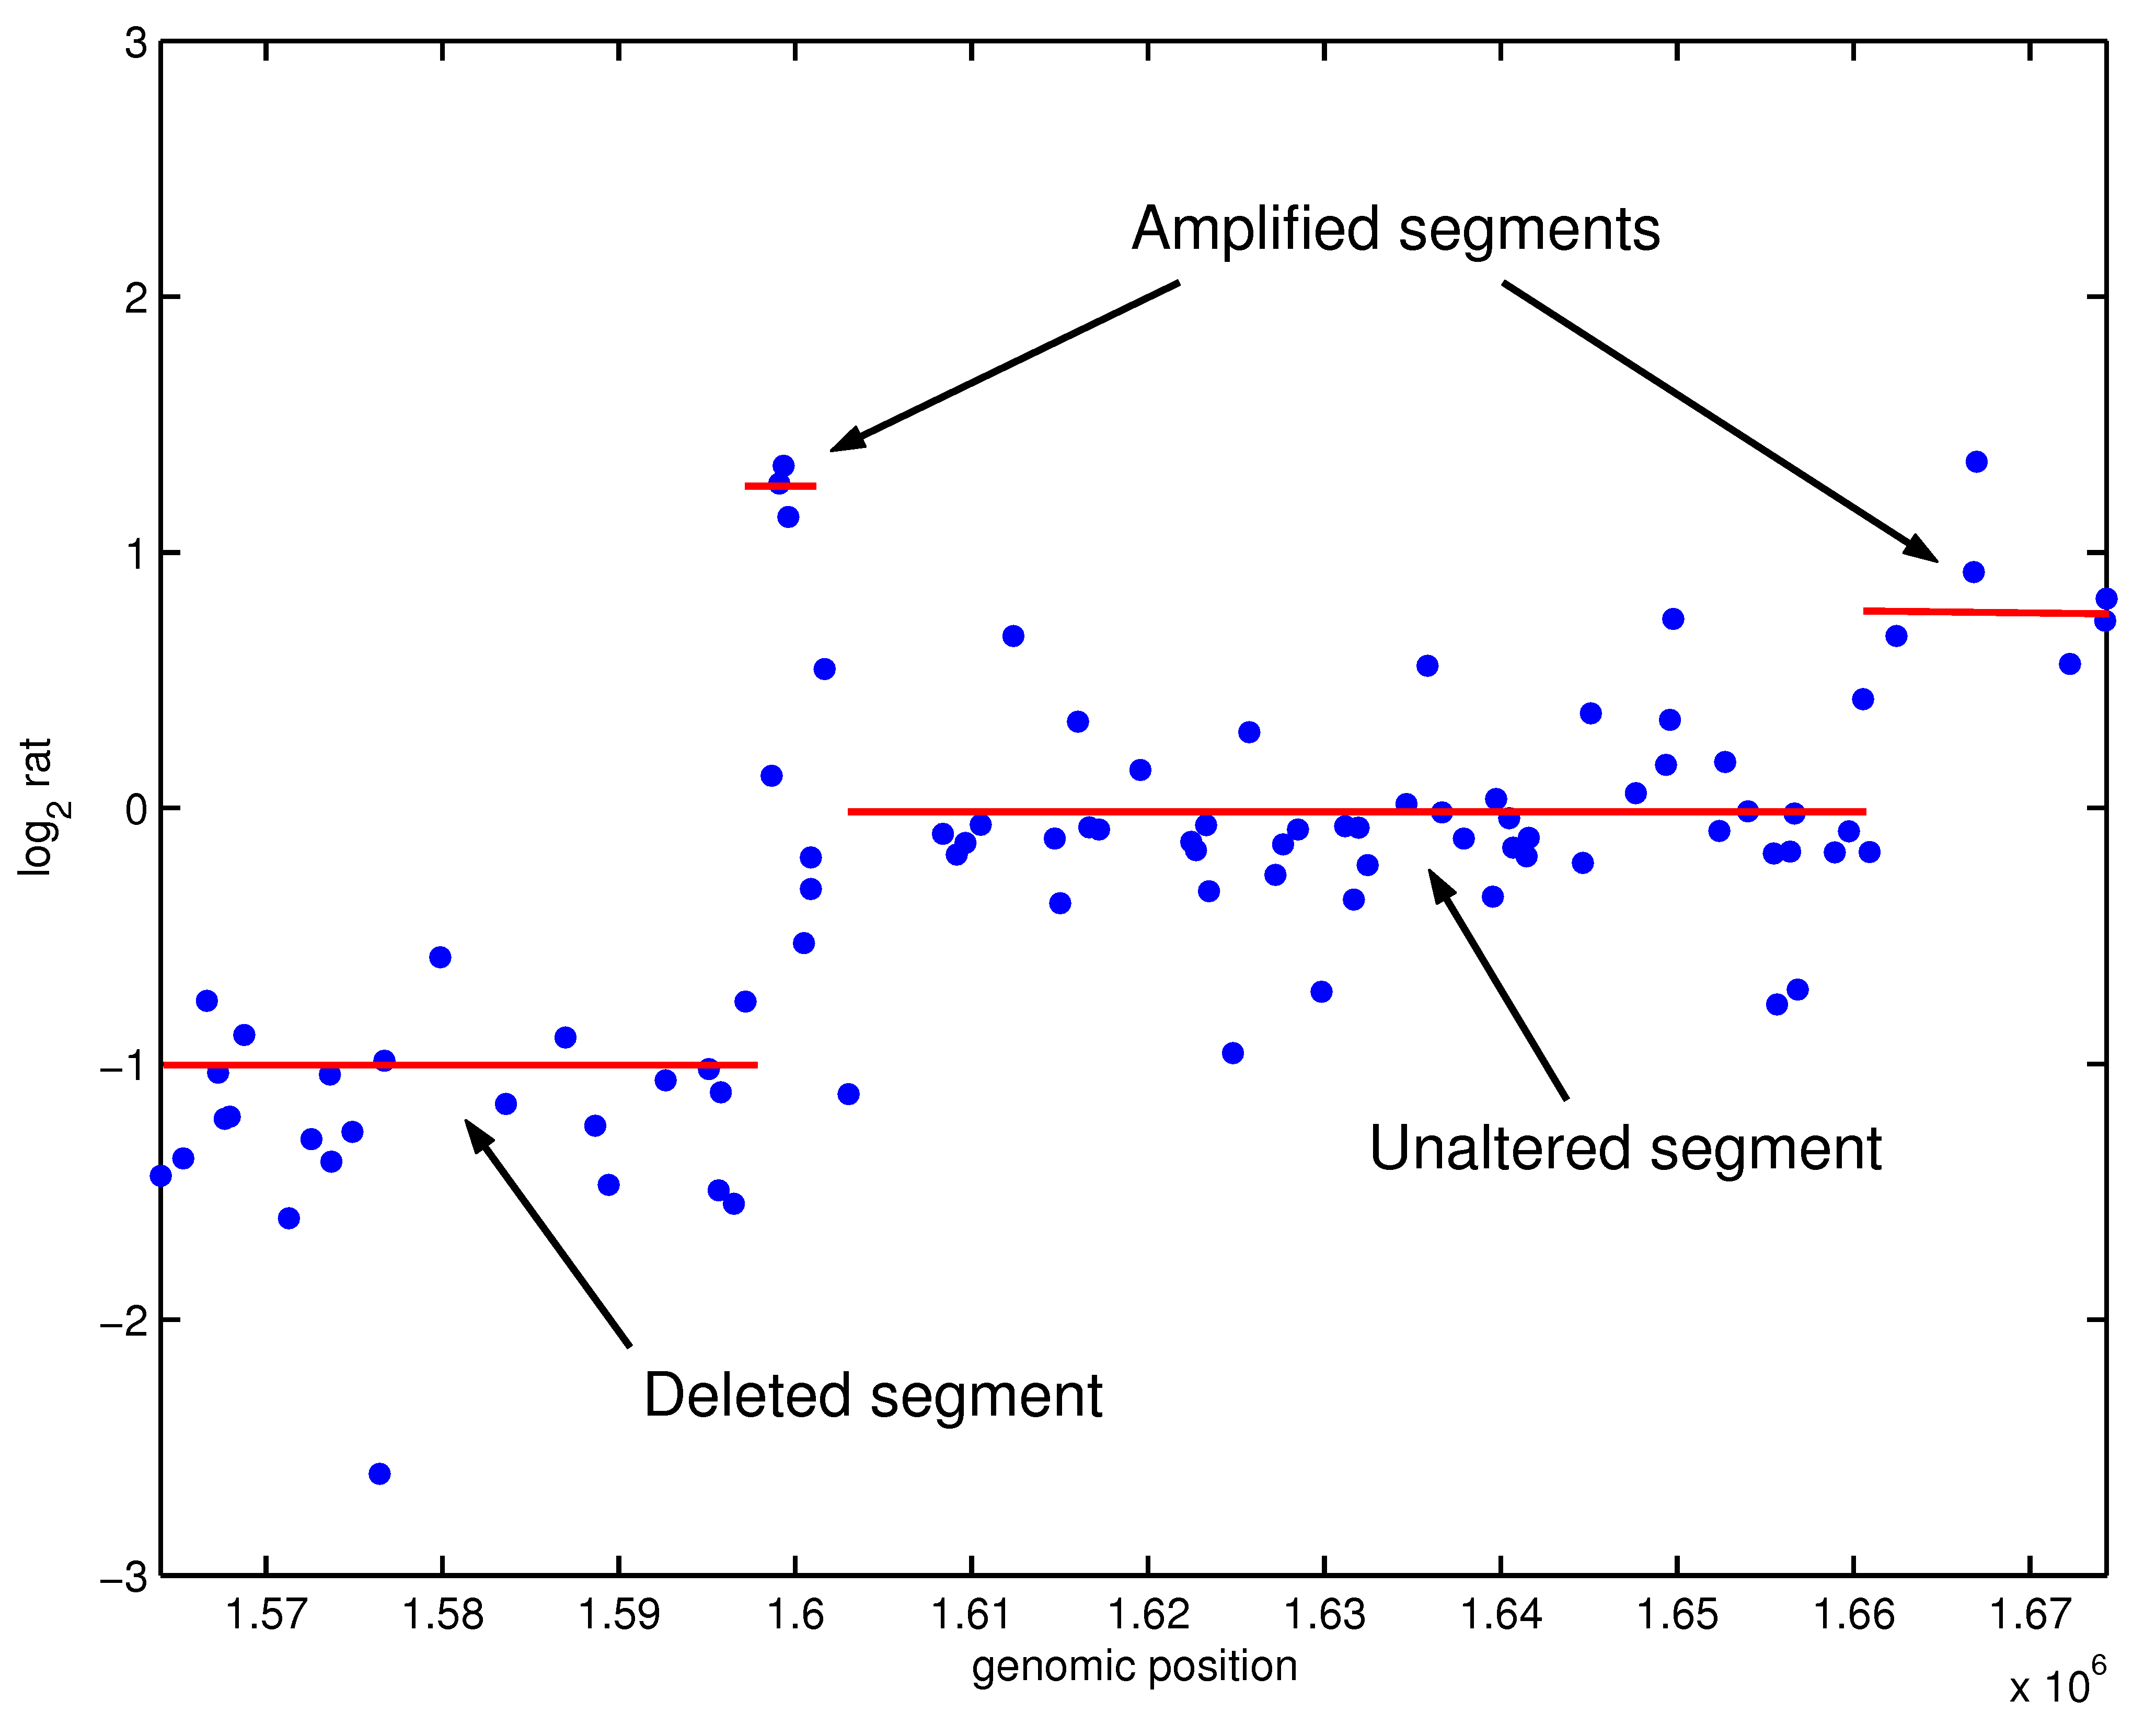
\epsfig{file = \fighd/profile_example.eps, clip=, scale=.325}
  \end{tabular} \\
  \refer{Pic05}
  }

%==================================================================== 
\frame{ \frametitle{Change-point model} 
  \emphase{Notations:}
  \begin{itemize}
  \item $K = $ number of segments \pause
  \item $r = $ region (or segment) $\llbracket \tau_r, \tau^r
    \rrbracket$; $n_r =$ length of $r$ \pause
  \item $m = $ segmentation: $m = \{r_1, \dots, r_K: \tau_{r+1} =
    \tau^r +1\}$ \pause
  \item $Y_t = $ signal at position $t$ ($t \in \llbracket 1, n
    \rrbracket$); $\Ybf = \{Y_t\}$. 
  \end{itemize}
  \bigskip\pause
  \emphase{Model:}
  \begin{itemize}
  \item $\{Y_t\}$ independent
  \item $t \in r$: 
    $$
    Y_t \sim p(\cdot | \theta_r)
    $$
  e.g. 
  $$
  p(\cdot|\theta_r) = \Ncal(\mu_r, \sigma^2), \qquad \Ncal(\mu_r,
  \sigma^2_r), \qquad \Pcal(\lambda_r)
  $$
  \end{itemize}
  \refer{PRL05}
  }

%====================================================================
\frame{ \frametitle{Inference}
%==================================================================== 
  \paragraph{Estimation of $\thetabf$ given $m$:} no specific
  problem, can rewritten as a (generallized) linear model:
  $$
  g(\Esp\Ybf) = \Zbf \thetabf.
  $$

  \pause
  \paragraph{General inference:} due to the
  \emphase{discontinuity of $p(\Ybf|m, \thetabf)$} with respect to
  $m$, standard MLE properties do not apply to
  $(\widehat{\thetabf}, \widehat{m})$.  \\
  \ra Inference (e.g.  confidence interval) of the breakpoints is
  not standard.
  
  \bigskip\pause
  \paragraph{Gaussian context:} \Refer{Bai and Perron (1998,
    2003)}\nocite{BaP98,BaP03} proved the consistency of the
  least-square estimates of
  \begin{itemize}
  \item $\widehat{\tau}_k$ at rate $1/n$
  \item $\widehat{\thetabf}$ at rate $1/\sqrt{n}$, with asymptotic normality.
  \end{itemize}
  Other consistency results in \refer{LaM00}.
  }

%==================================================================== 
\subsection{Model selection}
%==================================================================== 
\frame{ \frametitle{Model selection: Choice of $K$}
  \paragraph{Penalised contrast: 2 steps} \pause \\
  %\hspace{-0.5cm}
  \begin{tabular}{p{0.45\textwidth}p{0.5\textwidth}}
    \emphase{1:} Best segmentation within $\Mcal_K$ & 
    $
    \widehat{m}(K) = \arg\min_{m \in \Mcal_K} \ell(\Ybf, m)
    $ \pause \\
    \\ 
    \emphase{2:} Best dimension $K$ & 
    $
    \widehat{K} = \arg\min_{K} \ell(\Ybf, \widehat{m}(K)) + \pen(K)
    $
  \end{tabular}

  \bigskip\pause
  \paragraph{Examples:} \\
  \begin{tabular}{p{0.3\textwidth}p{0.5\textwidth}}
    \refer{Leb05}: & $\pen(K) = f(|\Mcal_K|);$ \\
    \\
    \refer{Lav05}: & $\pen(K) = \beta K.$ \\
  \end{tabular}

  \bigskip\pause
  \begin{itemize} 
  \item \emphase{Constant penalty} within each dimension $\Mcal_K$.
  \item The best model \emphase{$\widehat{m}(K)$ does not depend} on
    the penalty $\pen(K)$.
  \item Some (very sensitive in practice) constants need to be tuned.
  \end{itemize}
  }

%====================================================================
\frame{ \frametitle{Model selection : BIC}
  The standard Laplace approximation used in 
  $$
  \log p(M | \Ybf) = \log \int p(M, \theta | \Ybf) \dd \theta
  \approx \log p(M | \Ybf, \widehat{\theta}) - \frac{\log n}2 \dim(M)
  %=:  \BIC(M)
  $$
  does not hold when the 'model' $M$ refers to the dimension $K$ since
  $$
  \Mcal_K = \bigcup_{m\ \in \Mcal_K} \text{span}(m).
  $$

  \bigskip\pause
  \paragraph{Modified BIC.} Based on uniform prior distribution of the
  breakpoints, \refer{ZhS07} study the behaviour of
  $$
  B_t = S_t - t S_n /n, \quad \text{where } S_t = \sum_{i=1}^t Y_i
  $$
  and derive 
  $$
  \pen(K) = f(|\Mcal_K|) + g\left(\emphase{\sum_{r \in \widehat{m}(K)}
      \log n_r}\right)
  $$
  }

% %==================================================================== 
% \frame{ \frametitle{Example: BT474 cell line, chromosome 1} 
%   \paragraph{Adaptive choice of the number of segments.} :
%   $$
%   \begin{tabular}{cc}
%     Homogeneous variances & Heterogeneous variances \\
%     $\widehat{K} = 10$  segments & $\widehat{K} = 2$ segments \\
%     \epsfig{file = \fighd/bt474_c1_seg_homo_K10.eps, clip=, width=0.4\textwidth} &
%     \epsfig{file = \fighd/bt474_c1_seg_hetero_K2.eps, clip=, width=0.4\textwidth} \\
%   \end{tabular}
%   $$
%   Homogeneous variances result in smaller segments.
%   }

%==================================================================== 
\subsection{Optimal segmentation}
%==================================================================== 
\frame{ \frametitle{Optimal segmentation} 
  For a given dimension $K$, the optimal segmentation has to be found
  within 
  $$
  \Mcal_K = \{m: |m| = K\},
  \qquad |\Mcal_K| = \binom{n-1}{K-1}
  $$ \pause

  \paragraph{Consequences.}
  \begin{itemize}
  \item \emphase{Exhaustive search} can not be achieved. \pause
  \item \emphase{Dynamic programming} provides maximum likelihood
    $(\widehat{m}, \widehat{\thetabf})$ with complexity $\Ocal(K
    n^2)$. \pause
  \item \emphase{Lasso} criterion can be applied (\refer{TiW08}):
    $$
    \arg\min_m \sum_k \sum_{t \in r_k} (Y_t - \mu_k)^2 + \lambda
    \sum_k |\mu_k - \mu_{k-1}|
    $$
    with linear complexity (\refer{HaL08}).
  \end{itemize}
  }

%==================================================================== 
\frame{ \frametitle{Dynamic programming} 
  \paragraph{Segment cost:} for segment $r = \llbracket i, j
  \rrbracket$, 
  $$
  C(r) = - \log P(Y^r | \widehat{\theta}^r)
  $$ 
  \bigskip\pause
  \paragraph{Optimal segmentation:} recall that $m = \{r_1, \dots, r_K\}$, 
  $$
  \widehat{m} = \arg\min_{m \in \Mcal_K} \sum_k C(r_k)
  $$
  \bigskip\pause
  \paragraph{Optimal segmentation in $K=2$:}
  $$
  S_2(1, n) = \min_{1 < t < n} C(1, t) + C(t+1, n)
  $$
  \bigskip\pause
  \paragraph{Optimal segmentation in $K$:}
  $$
  S_K(1, n) = \min_{K-1 < t < n} S_{K-1}(1, t) + C(t+1, n)
  $$ 
  }

%====================================================================
\frame{ \frametitle{Computational point of view}
  \paragraph{Overall complexity:} Dynamic programming has a
  $\Ocal(n^2)$ complexity because there is a \emphase{quadratic number
    of segments} to be considered.

  \bigskip\pause
  \paragraph{Linear algebra:} The dynamic programming recursion can be
  viewed as a \emphase{scalar product} $\Rightarrow$ For all
    function $F(m)$
  $$
  F(m) = \prod_{r \in m} f(r).
  $$\pause
  Letting $\mathbf{A}: (n+1) \times (n+1)$:
  $$
  \begin{array}{rclll}
    {\bf A}_{ij} & = & f(\llbracket i, j \llbracket ) & \quad & \text{if } 1
    \leq i < j \leq n+1 \\
    & = & 0 & & \text{otherwise.}
  \end{array}
  $$\pause
  Then, \emphase{all terms} for $1 \leq k \leq K$, $1 \leq j \leq
  n+1$,  
  $$
  \sum_{m \in \Mcal_k(\llbracket 1, j\llbracket)} F(m) = (\mathbf{A}^k)_{1,j}
  $$
  can be computed in \emphase{$O(K n^2)$}.  
  }


%==================================================================== 
\subsection{Exploring the segmentation space}
%====================================================================
\frame{ \frametitle{Exploring the segmentation space: Bayesian framework}
  \vspace{-1cm}
  \begin{description}
  \item[$p(K) = $] prior of dimension $K$;\pause
  \item[$p(m|K) = $] prior of segmentation $m$ given dimension $K$,
    $$
    \text{for example:} \qquad
    p(m|K) = 1 \left/ |\Mcal_K| \right.
    $$
    that is, \emphase{uniform prior} within each dimension;\pause
  \item[$p(m) = $] prior of segmentation $m$,
    $$
    \text{for example:} \qquad
    p(m) \propto \prod_{r \in m} n_r
    $$
    that favours \emphase{regularly spaced} change-points
    ($\rightarrow$ implicit prior on $K$);\pause
  \item[$p(\theta|m) =$] prior of $\theta$ given segmentation $m$.
  \end{description}
  \refer{RLR09}
  }

%==================================================================== 
\frame{ \frametitle{Summing over all segmentations}
  \paragraph{Under a factorisation assumption:}
  $$
  p(m) = \prod_{r \in m} f(r), 
  \quad
  p(\theta|m) = \prod_{r \in m} f(\theta_r) 
  \quad
  p(\Ybf|m, \theta) = \prod_{r \in m} f(Y^r, \theta_r) 
  $$
  (not true for homoscedastic models), \pause \emphase{'integral'
    sums can be rewritten} as
  $$
  \sum_{m \in \Mcal_K} f(m) = \sum_{m \in \Mcal_K} \prod_{r \in m} f(r)
  $$

  \bigskip\pause
  \paragraph{Total probability:}
  $$
  p(\Ybf|K) = \sum_{m \in \Mcal_K} \prod_{r\in m} \int p(Y^r|\theta_r) p(\theta_r)
  \dd \theta_r = \sum_{m \in \Mcal_K} \prod_{r\in m} p(Y^r)
  $$

  \pause
  \paragraph{Localisation of the $k$-th breakpoint:}
  \begin{eqnarray*}
    \Pr\{\tau_k = t | K, \Ybf\} & \propto & \left(\sum_{m \in \Mcal_k(1, t)} \prod_{r
    \in m} p(Y^r)\right) \left(\sum_{m \in \Mcal_{K-k}(t+1, n)} \prod_{r
    \in m} p(Y^r)\right)
  \end{eqnarray*}
%   \emphase{Conjugate priors.} $\theta^0_r =$ parameter
%     of the prior $p(\theta_r)$
%     $$
%     f(Y^r; \theta^0_r) = \int p(Y^r|\theta_r) p(\theta_r; \theta^0_r) \dd_r
%     \quad \text{has an explicit form.}
%     $$
%     Avoids the Laplace approximation: \\
%     $\rightarrow$ regularity conditions \emphase{are fulfilled} for
%     any segmentation $m$, \\
%     $\rightarrow$ but the asymptotic framework does not apply to small regions.
  }

%====================================================================
\frame{ \frametitle{Exploring the segmentation space}
  We are hence able to \emphase{compute in $O(Kn^2)$}, \pause
  \begin{itemize}
  \item The probability that there is a \emphase{breakpoint at
      position $t$}:
    $$
    \Pr\{\exists k: \tau_k = t | \Ybf, K\} = \sum_{k=1}^K \Pr\{\tau_k = t
    | K\}
    $$ \pause
  \item The probability for a \emphase{segment $r = \llbracket t_1,
      t_2 \llbracket$ to be part of segmentation}
    $$
    \Pr\{r \in m | \Ybf, K\} = \sum_{k=1}^K \Pr\{\tau_k=t_1, \tau_{k+1}=t_2
    | \Ybf, K\};
    $$ \pause
  \item The \emphase{posterior entropy of $m$} within a dimension:
    $$
    \Hcal(K) = - \sum_{m \in \Mcal_K} p(m|\Ybf, K) \log p(m|\Ybf, K) 
    $$\pause
  \end{itemize}   
  \paragraph{Similar to} an algorithm proposed by \refer{Gue07} in the HMM
  context with known parameters.

 }

%====================================================================
\frame{ \frametitle{A CGH profile: $K = 3, 4$}
  \vspace{-.25cm}
  \begin{tabular}{lll}
    \hspace{-0.5cm}
    \begin{tabular}{p{0.2\textwidth}} Optimal segmentation \end{tabular}
    &
    \hspace{-0.5cm}
    \begin{tabular}{c}
      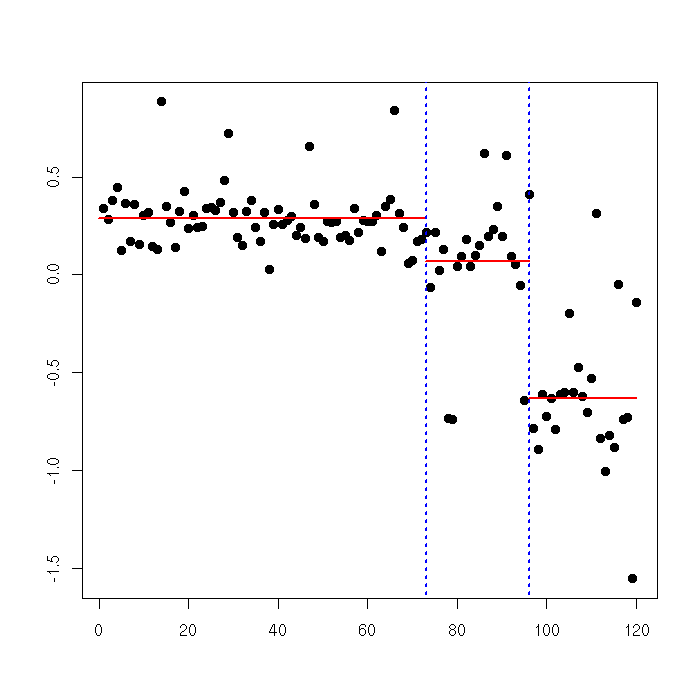
\includegraphics[width=0.35\textwidth, height=0.3\textheight,
      clip=]{\fighd/CopyNumberChr10_BIC}   \pause
    \end{tabular}
    &
    \hspace{-0.5cm}
    \begin{tabular}{c}
      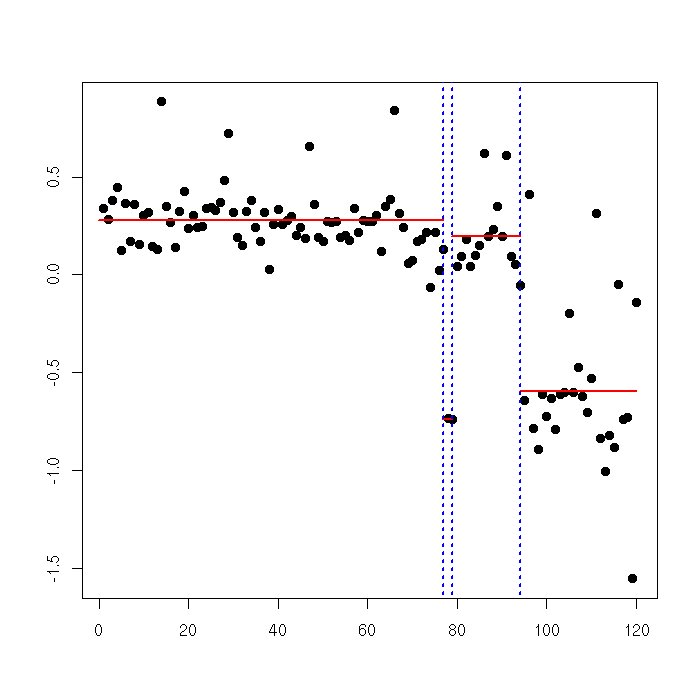
\includegraphics[width=0.35\textwidth, height=0.3\textheight,
      clip=]{\fighd/CopyNumberChr10_ICL}  
    \end{tabular} \pause\\ 
    \hspace{-0.5cm}
    \begin{tabular}{p{0.2\textwidth}} Breakpoint position \end{tabular}
    &
    \hspace{-0.5cm}
    \begin{tabular}{c}
      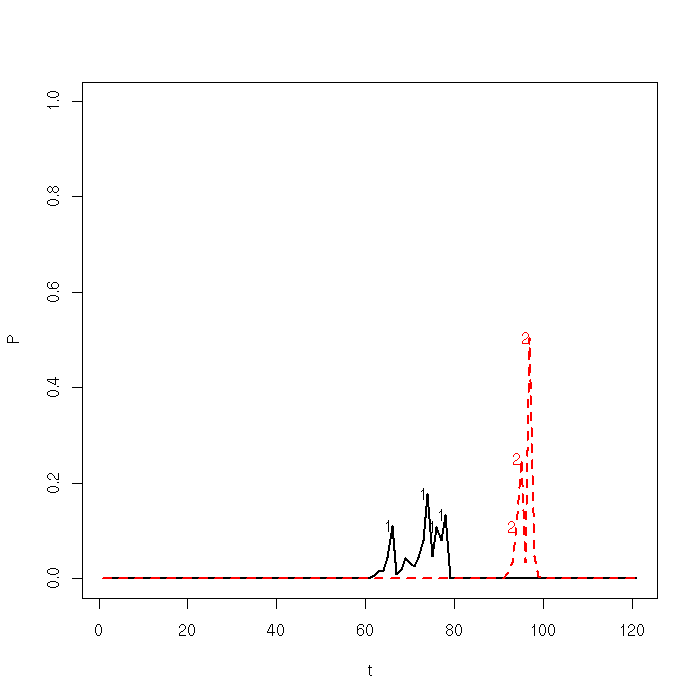
\includegraphics[width=0.35\textwidth, height=0.3\textheight,
      clip=]{\fighd/CopyNumberChr10_ProbaBIC}   \pause
    \end{tabular}
    &
    \hspace{-0.5cm}
    \begin{tabular}{c}
      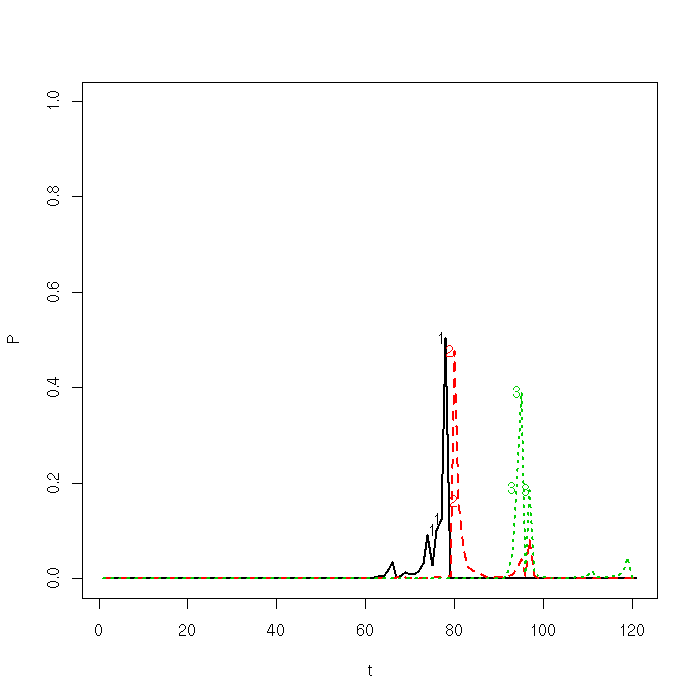
\includegraphics[width=0.35\textwidth, height=0.3\textheight,
      clip=]{\fighd/CopyNumberChr10_ProbaICL}  
    \end{tabular} \pause\\ 
    \hspace{-0.5cm}
    \begin{tabular}{p{0.2\textwidth}} Segment probability \end{tabular}
    &
    \hspace{-0.5cm}
    \begin{tabular}{c}
      \vspace{-.5cm}
      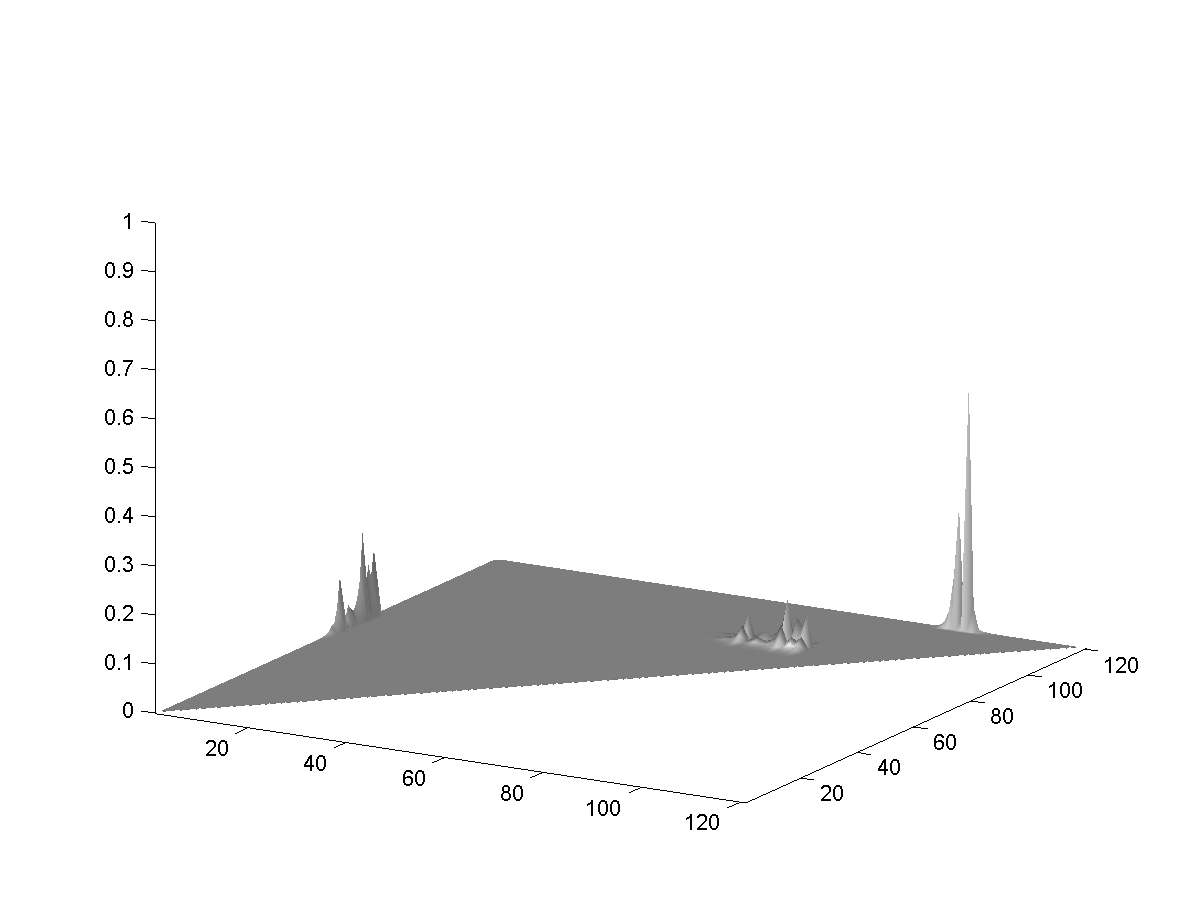
\includegraphics[width=0.35\textwidth, height=0.35\textheight,
      clip=]{\fighd/ProbSeg-BIC}     \pause
    \end{tabular}
    &
    \vspace{-.5cm}
    \begin{tabular}{c}
      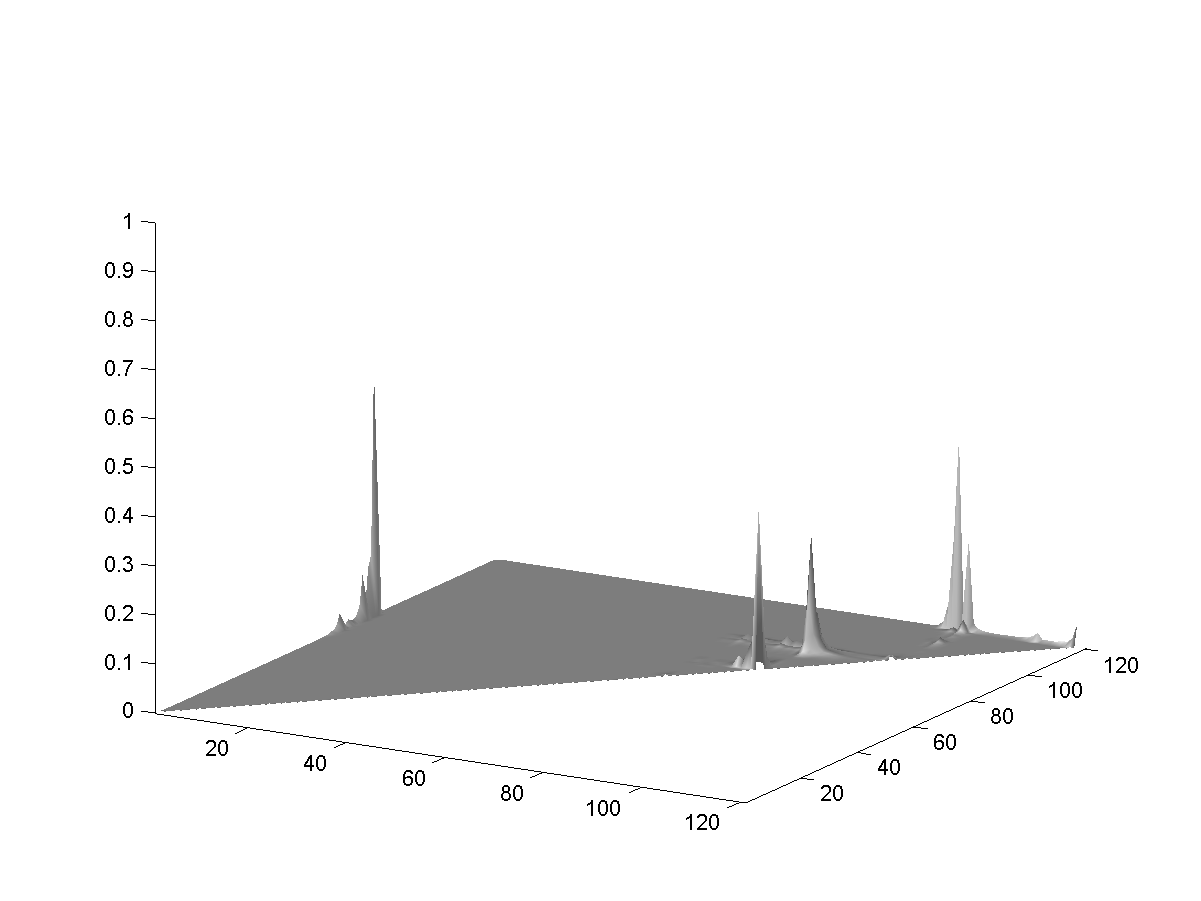
\includegraphics[width=0.32\textwidth, height=0.27\textheight,
      clip=]{\fighd/ProbSeg-ICL}   
    \end{tabular} 
  \end{tabular}
  }

%====================================================================
\frame{ \frametitle{Back to model selection: Exact BIC}
  The conditional probabilities of the dimension and of the
  segmentation also involve 'integral' sums.\pause

  \bigskip
  \paragraph{Choice of $K$.}
  $$
  \BIC(K) = \log p(\Ybf, K) = \log \left[\emphase{\sum_{m \in
        \Mcal_K}} p(m) \int p(\Ybf | m, \theta) p(\theta |m) \dd
    \theta \right].
  $$
  \bigskip\pause
  \paragraph{Choice of $m$.}
  $$
  \BIC(m) = \log p(\Ybf, m) = \log \left[p(m) \int p(\Ybf | m,
    \theta) p(\theta |m) \dd \theta \right]
  $$
  where $p(m)$ must be normalised so that
  $$
  \sum_K \emphase{\sum_{m \in \Mcal_K}} p(m) = 1.
  $$
  }

%====================================================================
\frame{ \frametitle{Exact ICL criterion}
  \emphase{Incomplete data model context} (mixture model):
  \begin{itemize}
  \item \refer{BCG00} add an entropy term $\Hcal(K)$ to the $\BIC(K)$
    penalty
  \item $\Hcal(K)$ accounts for the reliability of the prediction of
    the latent variable.
  \end{itemize}
  \bigskip \pause
  \emphase{Segmentation context.}
  \begin{itemize}
  \item Change-point positions can be viewed as \emphase{latent
      variables}.\pause 
  \item For a given dimension $K$, it is desirable that the best
    segmentation \emphase{clearly outperforms the others}:
    $$
    \text{for any } m \in \Mcal_K \setminus \{\widehat{m}(K)\}:
    \quad p(\widehat{m}(K)|\Ybf) \gg p(m | \Ybf).\pause
    $$
  \item This can be measured by the \emphase{posterior entropy $\Hcal(K)$}.
  \end{itemize}
  \bigskip
  \emphase{ICL criterion:}
  $$
  \ICL(K) = \log \sum_{m \in \Mcal_K} p(\Ybf, m) - \Hcal(K)
  $$
    }

%====================================================================
\frame{ \frametitle{Comparison BIC/ICL: Simulation study}
  \begin{columns}
    \begin{column}{0.45\linewidth}
      \emphase{Simulations: } Poisson signal with alternating
      means $\lambda_0$ and $\lambda_1$, $n = 100$. \\
      \bigskip \emphase{Criterion} = \% of recovery of the true number
      of segments ($K =
      5$). \\
      \bigskip
      \begin{itemize}
      \item $\BIC(m)$ achieves (much) better performances than
        $\BIC(K)$
      \item $\ICL(K)$ outperforms both $\BIC(K)$ and $\BIC(m)$.
      \end{itemize}
    \end{column}
    
    \begin{column}{0.45\linewidth}
      \begin{tabular}{c}
        \textcolor{green}{$\BIC(K)$} \quad \textcolor{red}{$\BIC(m)$} \quad
        \textcolor{blue}{$\ICL(K)$} \\
        ~\\
        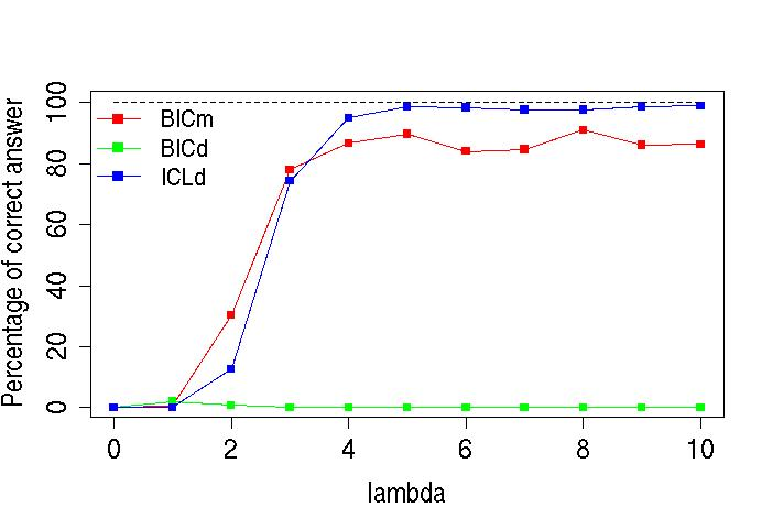
\epsfig{file=\fighd/ICLvsBIC.ps, clip=, bbllx=50, bblly=60,
          bburx=545, bbury=340, width=.9\textwidth,
        height=.5\textheight} \\ 
        $\lambda_1 - \lambda_0$ ($\lambda_0 = 1$)
      \end{tabular}
    \end{column}
  \end{columns}
 }

%====================================================================
\frame{ \frametitle{}
  \vspace{-1cm}
  $$
  \begin{tabular}{cc}
    \begin{tabular}{c}
      \emphase{\large Back to the example} \\
      \epsfig{file=\fighd/CopyNumberChr1_Alone.ps, 
        bbllx=38, bblly=40, bburx=565, bbury=385, width=4.25cm, height=2.25cm,
        clip=} \\
      \\
      $\BIC(K) \rightarrow \widehat{K} = 10$ \\
      \epsfig{file = \fighd/BIC2_NP.ps,
      width=5cm, height=2.5cm, clip=} \\
    \end{tabular}
    &
    \begin{tabular}{c}
%       \\
%       $\ICL(K) = f[\BIC(K)]$ \\
%       \epsfig{file=\fighd//BICandEntropy.ps,
%       clip=, scale=0.25, bbllx=38, bblly=40, bburx=565, bbury=385}    
      $\BIC(m) \rightarrow \widehat{K} = 3$ \\
%      \epsfig{file = \fighd/BIC_NP.ps,
      \epsfig{file = \fighd/ICL_NP.ps,
      width=5cm, height=2.5cm, clip=} \\
      \\
      $\ICL(K) \rightarrow \widehat{K} = 4$ \\
%      \epsfig{file = \fighd/ICL_NP.ps,
      \epsfig{file = \fighd/BIC_NP.ps,
      width=5cm, height=2.5cm, clip=} \\
    \end{tabular}
  \end{tabular}
  $$
  When $K$ exceeds the 'true' dimension, all segmentations
  nested within the 'true' one have a high posterior probability,
  which increases the entropy. 
}

%====================================================================
\frame{ \frametitle{Conclusions and open problem}
  \paragraph{Statistical inference of change-point models} is not
  standard due to the discontinuity of the likelihood. \\
  Choosing the right number of breakpoints is also a practical issue.

  \bigskip\pause
  \paragraph{Dynamic-programming-like} algorithms allow us to explore
  the whole segmentation space with quadratic complexity.

  \bigskip\pause
  \paragraph{In a Bayesian settings} exact credibility intervals,
  posterior distribution over the segmentation space or dimension can
  then be calculated.

  \bigskip\pause
  \paragraph{In genomics, new sequencing technologies} dramatically
  augmented the resolution ($n$), so quadratic complexity is out of reach.\\
  \ra A partial exploration of the most probable segmentations may be
  more reasonable.

  }

%====================================================================
{\tiny
  \bibliography{/Biblio/ARC,/Biblio/AST,/Biblio/SSB}
  \bibliographystyle{/Latex/astats}
  %\bibliographystyle{plain}
  }

%====================================================================
%====================================================================
\end{document}
%====================================================================
%====================================================================
